\graphicspath{{chapters/14/images}}
\chapter{Quantifying uncertainties and sampling quality}

\section{Introduction}

	\subsection{Key definitions}
	Expectation value:

	$$\langle x\rangle = \int xP(x)dx = \sum\limits_jx_jP(x_j)$$

	Estimate: arithmetic mean:

	$$\bar{x} = \frac{1}{n}\sum\limits_{j=1}^nx_j$$

	Variance:

	$$\sigma^2_x = \int dxP(x)(x-\langle x\rangle)^2 = \sum\limits_{j}P(x_j)\bigl(x_j-\langle x\rangle\bigr)^2$$

	Standard deviation $\sigma_x$, its estimate is the experimental standard deviation:

	$$s(x) = \sqrt{\frac{\sum\limits_{j=1}^n(x_j-\bar{x})^2}{n-1}}$$

	Linearly uncorrelated observables:

	$$\bigl\langle(x-\langle x\rangle)(y-\langle y\rangle)\bigr\rangle = 0$$

	Experimental standard deviation of the mean: $s(\bar{x}) = \frac{s(x)}{\sqrt{n}}$ if the $x_j$ are assumed to be linearly uncorrelated.
	The correlation time $\tau$: the longest separation tiem $\Delta t$ over which $x(t)$ and $x(t + \Delta t)$ remain linearly correlated.
	The two-sided confidence interval: $\langle x\rangle = \bar{x} \pm U$ with $U = ks(\bar{x})$ and $k$ the coverage factor for a given level of confidence $p$ expressed in percentage.

	\subsection{Time scales}

	\begin{figure}[H]
		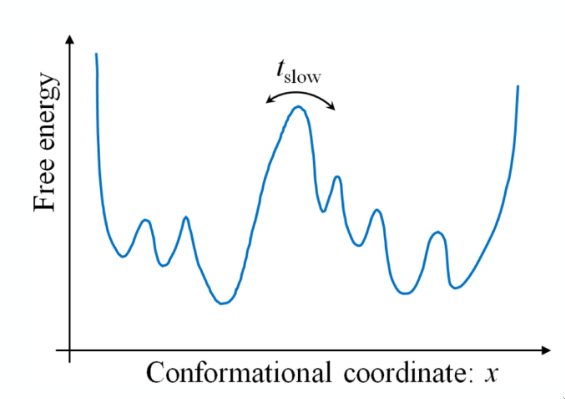
\includegraphics[width = \textwidth]{time-scales}
		\caption{Time scales}
		\label{fig:time-scales}
	\end{figure}

\section{Equilibration}
Time series of scalar values:

\begin{multicols}{2}
	\begin{itemize}
		\item System size.
		\item Membrane area.
		\item Potential energy or total energy.
		\item Temperature in the NVE ensemble.
		\item Density in the NPT ensemble.
		\item Pressure.
		\item Radius of gyration.
		\item Configurational distance measures like RNMS, all-to-all RMSD map.
			Considering RMSD:

			$$RMSD(\vec{r}, \vec{s}) = \sqrt{\frac{1}{N}\sum\limits_{i=1}^N|\vec{r}_i-\vec{s}_i|^2}$$
	\end{itemize}
\end{multicols}

\begin{multicols}{2}

	\begin{figure}[H]
		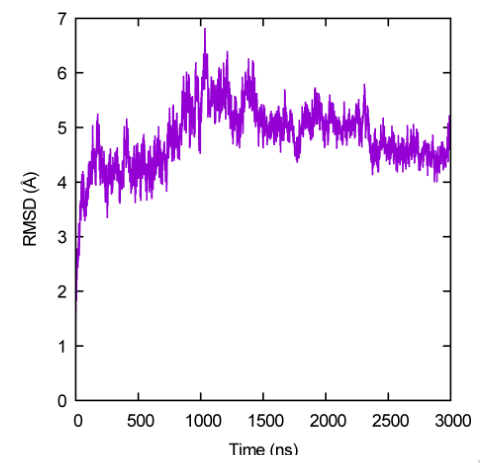
\includegraphics[width = 0.45\textwidth]{rmsd}
		\caption{RMSD}
		\label{fig:rmsd}
	\end{figure}

	\columnbreak

	\begin{figure}[H]
		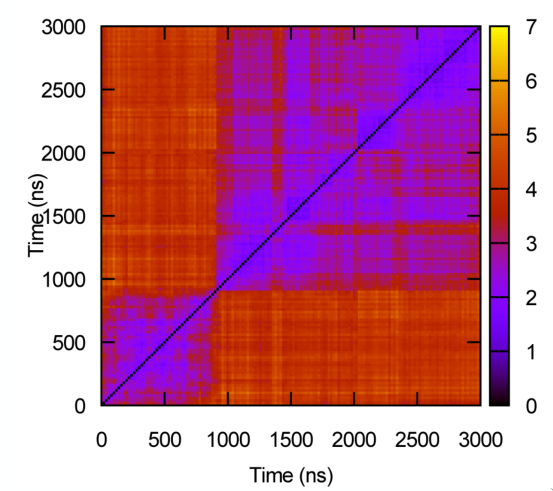
\includegraphics[width = 0.45\textwidth]{all-to-all-rmsd}
		\caption{All-to-all RMSD map}
		\label{fig:all-to-all-rmsd}
	\end{figure}

\end{multicols}

	\subsection{Qualitative behaviour}

	\begin{figure}[H]
		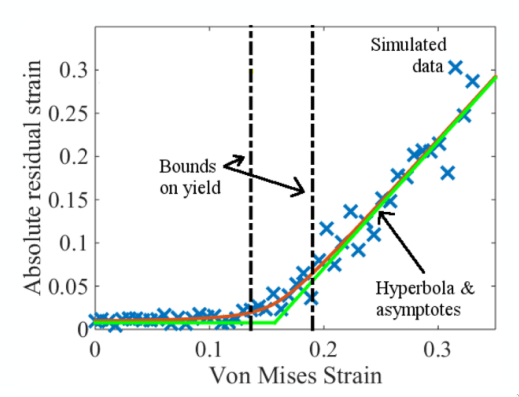
\includegraphics[width = \textwidth]{qualitative-behaviour}
		\caption{Qualitative behaviour}
		\label{qualitative-behaviour}
	\end{figure}

	\subsection{Independent simulations}
	Autocorrelation analysis:

	$$C(x_k, x_{k+j}) \equiv\frac{\bar{(x_k-\bar{x})(x_{k+j}-\bar{x})}}{s^2(x)}\Rightarrow C_j$$

	Combined clustering as in \ref{fig:independent_simulation}.

	\begin{figure}[H]
		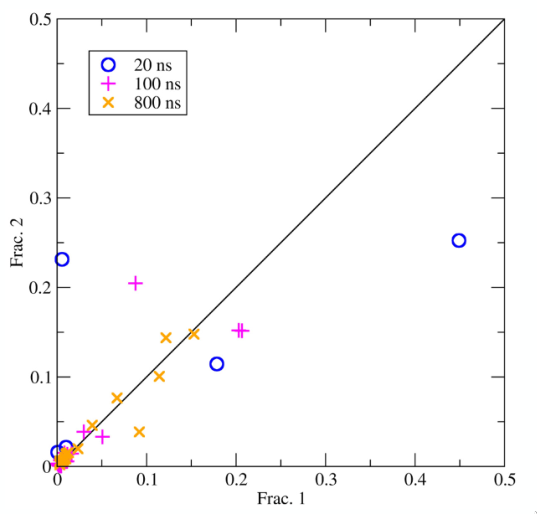
\includegraphics[width = \textwidth]{independent-simulations}
		\caption{Qualitative behaviour}
		\label{fig:independent_simulation}
	\end{figure}

	\subsection{Equilibration and production}

	\begin{figure}[H]
		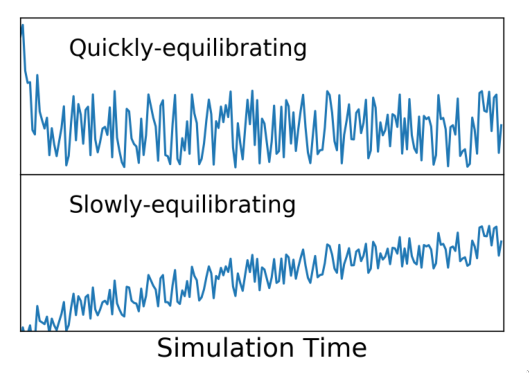
\includegraphics[width = \textwidth]{equilibration}
		\caption{Equilibration}
		\label{fig:equilibration}
	\end{figure}

	\begin{figure}[H]
		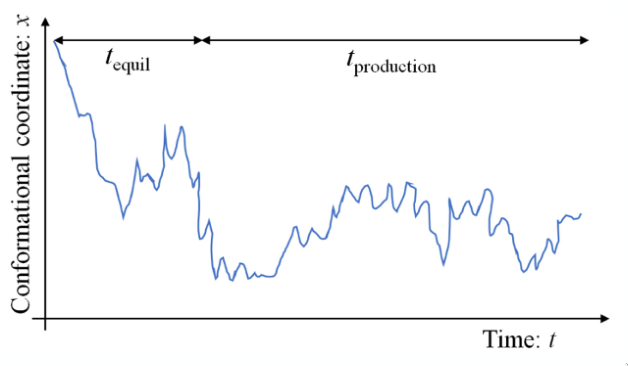
\includegraphics[width = \textwidth]{equilibration-production}
		\caption{Comparison of equilibration and production}
		\label{fig:equilibration-production}
	\end{figure}

	\subsection{Equilibration workflows}

	$$\overbrace{\underbrace{NVT}_{\substack{\text{short simulation to}\\\text{relax to temperature}\\\text{of interest}}}\rightarrow \underbrace{NVE}_{\text{short equilibration}}}^{\text{Suggested equilibration workflow}}\rightarrow \overbrace{NVE}^{\text{Production ensemble}}$$

	$$\overbrace{\underbrace{NVT}_{\substack{\text{short simulation to}\\\text{relax to temperature}\\\text{of interest}}}}^{\text{Suggested equilibration workflow}}\rightarrow \overbrace{\underbrace{NVT}_{\text{at known, fixed density}}}^{\text{Production ensemble}}$$

			$$\overbrace{\underbrace{NVT}_{\substack{\text{short simulation to}\\\text{relax to temperature}\\\text{of interest}}}\rightarrow \underbrace{NPT}_{\substack{\text{short simulation to}\\\text{relax to density of}\\\text{interest}}}\rightarrow\underbrace{NPT}_{\substack{\text{to compute average}\\\text{box size}}}\rightarrow \underbrace{NVT}_{\text{short equilibration}}}^{\text{Suggested equilibration workflow}}\rightarrow\overbrace{\underbrace{NVT}_{\substack{\text{for density defined by}\\\text{ pressure or unknown system}\\\text{density distribution,}\\\text{like a homogeneous system}}}}^{\text{Production ensemble}}$$

						$$\overbrace{\underbrace{NVT}_{\substack{\text{short simulation to}\\\text{relax to temperature}\\\text{of interest}}}\rightarrow \underbrace{NPT}_{\substack{\text{short simulation to}\\\text{relax to density of}\\\text{interest}}}}^{\text{Suggested equilibration workflow}}\rightarrow	\overbrace{NPT}^{\text{Production ensemble}}$$


\section{Autocorrelation}

	\subsection{Autocorrelation function}
	Observable $f(x)$.
	Autocorrelation function:

	$$C_f(t') = \frac{\bigl\langle(f(x)-\langle f\rangle)(f(t+t') - \langle f\rangle)\bigr\rangle}{\sigma^2_f}$$

	Time ordered sequence of values $f_j = f(t=j\Delta t)$:

	$$C_f(t') = \frac{1}{\sigma^2_f}\frac{1}{N}\sum\limits_{j=1}^{N-\frac{t'}{\Delta t}}(f(j\Delta t)-\langle f\rangle)(f(j\Delta t + t')-\langle f\rangle)$$

	\subsection{Autocorrelation time}
	Autocorrelation time:

	$$\tau_f = \int_0^{+\infty} dt' C_f(t')$$

	\begin{figure}[H]
		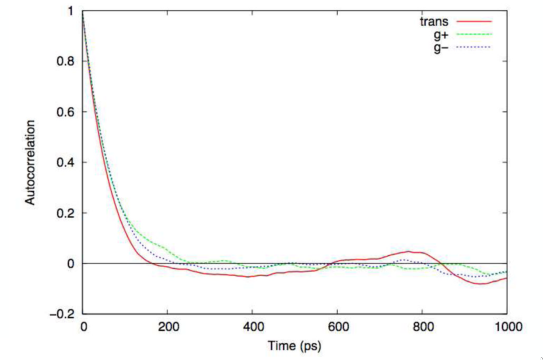
\includegraphics[width = \textwidth]{autocorrelation-time}
		\caption{Autocorrelation time}
		\label{fig:autocorrelation-time}
	\end{figure}

	The autocorrelation time $\tau_f$ is specific for each observable $f$ and allows to obtain the number of independent values of $f$ in the simulation:

	$$N_f^{ind}\simeq\frac{t_{sim}}{\tau_f}$$

	The standard deviation of the mean is:

	$$SE(f) = \frac{\sigma_f}{\sqrt{N_f^{ind}}}\sim\sigma_f\sqrt{\frac{\tau_f}{t_{sim}}}$$

	A confidence interval at $95\%$ implies: $\pm 2 SE(f)$.

\section{Block averaging analysis}
A trajectory with $N = M\cdot n$ snapshots is divided into $M$ segments of length $n$ with $n =1, 2, \dots$.
Compute $M$ averages:

$$\langle f\rangle_i, \qquad i = =1, \dots, M$$

Compute the standard deviation $\sigma_n$ for each value of $n$.
Running estimate of the overall standard error:

$$BSE(f, n) = \frac{\sigma_n}{\sqrt{M}}$$

For small values of $n$ and high values of $M$, the $BSE$ under-estimates the statistical error.
The $BSE$ is constant once the blocks are essentially independent of one another, or when the block length is substantially greater than the correlation time.


\begin{multicols}{2}

	\begin{figure}[H]
		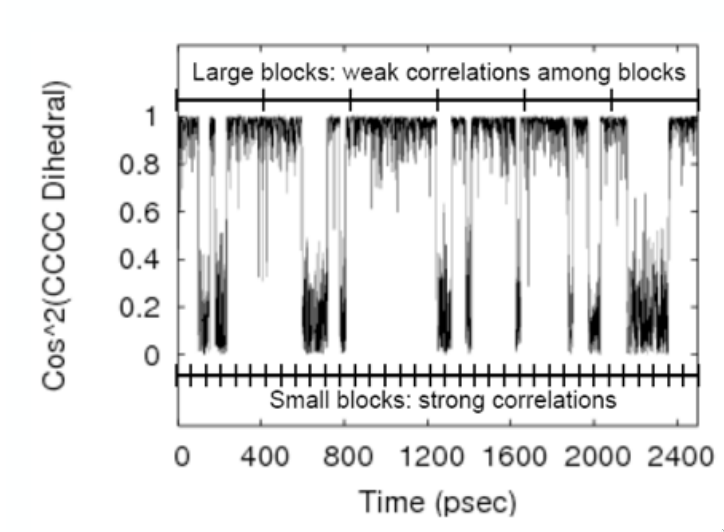
\includegraphics[width = 0.45\textwidth]{block-length}
		\caption{Varying block length}
		\label{fig:block-length}
	\end{figure}

	\columnbreak

	\begin{figure}[H]
		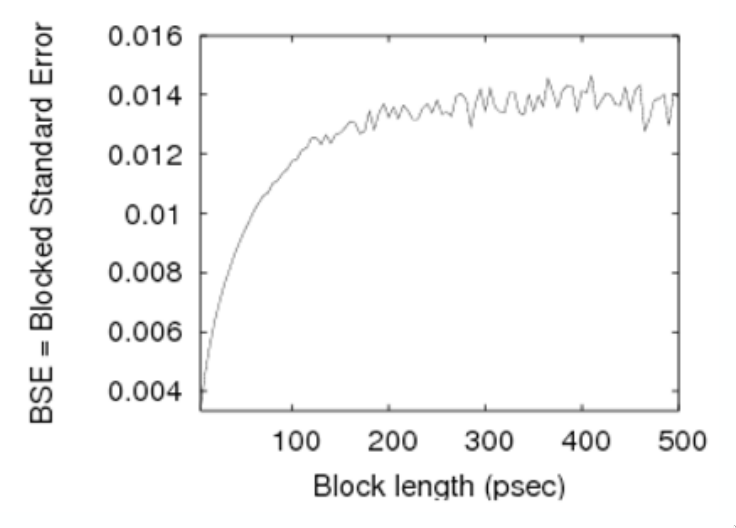
\includegraphics[width = 0.45\textwidth]{bse}
		\caption{BSE at varying block length}
		\label{fig:bse}
	\end{figure}

\end{multicols}
